\chapter{Технологическая часть}

В данном разделе производится выбор средств разработки программного обеспечения, раскрываются детали реализации и представляются способы взаимодействия с программным обеспечением. Также приводится листинг некоторых компонентов приложения. В частности рассмтриваются модели данных и приводится пример метода, с помощью которого осуществляется доступ к данным.


\section{Выбор СУБД}

СУБД --- это система управления базами данных. Так называют комплекс программно-языковых средств, позволяющих создавать базы данных и манипулировать данными \cite{7}.

Среди самых популярных реляционных СУБД можно выделить следующие:

\begin{itemize}
	\item MySQL --- СУБД с открытым исходным кодом. Является одной из самых популярных реляционных СУБД. Главное недостаток данной СУБД --- фрагментарное использование SQL;
	\item MS SQL Server --- СУБД, разрабатываемая компанией Microsoft. Основным недостатком является платный доступ и повышенное потребление ресурсов;
 	\item SQLite --- компактная встраиваемая СУБД с открытым исходным кодом. Недостатком является отсутствие системы пользователей, что недопустимо для поставленной задачи;
  	\item Oracle Database --- объектно-реляционная СУБД компании Oracle. Данная СУБД подходит для разнообразных рабочих нагрузок и может использоваться практически в любых задачах. Однако основными ее недостатками являются сложность в настраивании и повышенное потребление ресурсов;
   \item PostgreSQL --- современная СУБД с открытым исходным кодом. СУБД предоставляет транзакции со свойствами согласованности, изоляции, долговечности \cite{4}.
\end{itemize}

Для решения задачи была выбрана СУБД PostgreSQL, поскольку данная СУБД является наиболее развитой из открытых СУБД, кроме того Postgre проста в развертывании.

\section{Выбор языка программирования}
Для разработки серверной части был выбран язык программирования Java. Данный выбор обусловлен тем, что Java --- кросплатформенный, компилируемый язык программирования, поэтому разрабатанное ПО можно будет запустить на любой ОС.  

Для реализации REST API был выбран фреймворк Spring. Для коммуникации  серверной части приложения и базами данных была выбрана JPA спецификация.   

Для <<упаковки>> приложения в готовый продукт была выбрана система контейнеризации Docker \cite{8}.  

Тестирование программного обеспечения производилось с помощью фреймворка JUnit. С помощью данного фреймворка можно писать как модульные, так и функциональные тесты.  


\section{Детали реализации}

\newpage
В листинге \ref{lst:app1} представлена сущность базы данных --- Company.


\begin{lstlisting}[label=lst:app1, caption=Сущность Company, language=python]
package com.example.consensus.entities;

import com.fasterxml.jackson.annotation.JsonIgnore;
import lombok.Data;
import javax.persistence.*;
import javax.validation.constraints.NotBlank;
import javax.validation.constraints.Size;
import java.util.List;

@Table
@Entity
@Data
public class Company {
@Id
@GeneratedValue(strategy = GenerationType.IDENTITY)
private Long id;

@Column(name = "name")
private String name;

@Column(name = "logo")
private String logo;

@Column(name = "description")
private String description;

@Column(name = "ticker")
@NotBlank
@Size(min = 1, max = 6, message = "Ticker length may be between 1 and 6")
private String ticker;

@OneToMany(mappedBy = "companyForForecasts")
private List<Forecast> forecasts;

@OneToMany(mappedBy = "companyForNews")
private List<News> news;

@OneToOne(cascade =CascadeType.ALL)
@JoinColumn(name = "indicators_id", referencedColumnName = "id")
private Indicators indicators;

public void setFields(Company company) {
	setName(company.getName());
	setLogo(company.getLogo());
	setDescription(company.getDescription());
	setTicker(company.getTicker());
	setForecasts(company.getForecasts());
	setIndicators(company.getIndicators());
}
}	
\end{lstlisting}
\newpage

В листинге \ref{lst:app2} представлена сущность базы данных --- Forecast.


\begin{lstlisting}[label=lst:app2, caption=Сущность Forecast, language=python]
package com.example.consensus.entities;

import com.fasterxml.jackson.annotation.JsonIgnore;
import lombok.Data;
import javax.persistence.*;
import javax.validation.constraints.NotNull;
import java.sql.Timestamp;

@Table
@Entity
@Data
public class Forecast {
	@Id
	@GeneratedValue(strategy = GenerationType.IDENTITY)
	@NotNull
	private long id;

	@Column(name = "invest_house")
	private String investHouse;

	@Column(name = "date_publishing")
	private Timestamp datePublishing;

	@Column(name = "date_end")
	private Timestamp dateEnd;

	@Column(name = "date_update")
	private Timestamp dateUpdate;

	@Column(name = "goal_price")
	private int goalPrice;

	@Column(name = "forecast")
	private String forecast;

	@Column(name = "description")
	private String description;

	@ManyToOne
	@JoinColumn(name = "company_id", nullable = false)
	@JsonIgnore
	private Company companyForForecasts;

	public void setFields(Forecast forecast) {
		setInvestHouse(forecast.getInvestHouse());
		setDatePublishing(forecast.getDatePublishing());
		setDateEnd(forecast.getDateEnd());
		setDateUpdate(forecast.getDateUpdate());
		setGoalPrice(forecast.getGoalPrice());
		setForecast(forecast.getForecast());
		setDescription(forecast.getDescription());
		setCompanyForForecasts(forecast.getCompanyForForecasts());
	}
}
\end{lstlisting}

В листинге \ref{lst:app3} представлена сущность базы данных --- Indicators.

\begin{lstlisting}[label=lst:app3, caption=Сущность Indicators, language=python]
package com.example.consensus.entities;


import com.fasterxml.jackson.annotation.JsonIgnore;
import lombok.Data;
import javax.persistence.*;
import javax.validation.constraints.Min;
import javax.validation.constraints.NotNull;
import javax.validation.constraints.Size;

@Table
@Entity
@Data
public class Indicators {
	@Id
	@GeneratedValue(strategy = GenerationType.IDENTITY)
	@NotNull
	private long id;

	@Column(name = "price")
	@Min(value = 0, message = "Price can not be less then 0!")
	private double price;

	@Column(name = "market_cap")
	@Min(value = 0, message = "Market cap can not be less then 0!")
	private int market_cap;

	@Size(min = 0, max = 100, message = "Income must be expressed in %")
	@Column(name = "income")
	private int income;

	@Min(value = 0, message = "Revenue must be more then 0!")
	@Column(name = "revenue")
	private int revenue;

	@OneToOne(mappedBy = "indicators")
	@JsonIgnore
	private Company company;

	public void setFields(Indicators newIndicators) {
		setPrice(newIndicators.getPrice());
		setMarket_cap(newIndicators.getMarket_cap());
		setIncome(newIndicators.getIncome());
		setRevenue(newIndicators.getRevenue());
		setCompany(newIndicators.getCompany());
	}
}	
\end{lstlisting}

В листинге \ref{lst:app4} представлена сущность базы данных --- News.


\begin{lstlisting}[label=lst:app4, caption=Сущность News, language=python]
package com.example.consensus.entities;


import com.fasterxml.jackson.annotation.JsonIgnore;
import lombok.Data;
import javax.persistence.*;
import java.sql.Timestamp;

@Entity
@Table(name = "news")
@Data
public class News {
	@Id
	@GeneratedValue(strategy = GenerationType.IDENTITY)
	private Long id;

	@Column(name = "title")
	private String title;

	@Column(name = "date_public")
	private Timestamp datePublic;

	@Column(name = "content")
	private String content;

	@Column(name = "url")
	private String url;

	@Column(name = "author")
	private String author;

	@ManyToOne
	@JoinColumn(name = "company_id", nullable = false)
	@JsonIgnore
	private Company companyForNews;

	public void setFields(News news) {
		setAuthor(news.getAuthor());
		setContent(news.getContent());
		setUrl(news.getUrl());
		setCompanyForNews(news.getCompanyForNews());
		setDatePublic(news.getDatePublic());
		setTitle(news.getTitle());
	}
}
\end{lstlisting}

В листинге \ref{lst:app5} представлена сущность базы данных --- User.

\begin{lstlisting}[label=lst:app5, caption=Сущность User, language=python]
package com.example.consensus.entities;

import lombok.Data;
import javax.persistence.*;
import javax.validation.constraints.Email;
import java.util.Collection;

@Entity
@Data
@Table(name = "users")
public class User {

	@Id
	@GeneratedValue(strategy = GenerationType.IDENTITY)
	private Long id;

	@Column(name = "username")
	private String username;

	@Column(name = "password")
	private String password;

	@Email
	@Column(name = "email")
	private String email;

	@Column(name = "name")
	private String name;

	@Column(name = "surname")
	private String surname;

}
\end{lstlisting}

В листинге \ref{lst:app6} представлена сущность базы данных --- Role.

\begin{lstlisting}[label=lst:app6, caption=Сущность Role, language=python]
package com.example.consensus.entities;

import lombok.Data;
import javax.persistence.*;

@Entity
@Table(name = "roles")
@Data
public class Role {
	@Id
	@GeneratedValue(strategy = GenerationType.IDENTITY)
	private Long id;

	@Column(name = "name")
	private String name;
}	
\end{lstlisting}

В листингах \ref{lst:control1} -- \ref{lst:control2} приведены примеры взаимодействия клиента с сервером.

\begin{lstlisting}[label=lst:control1, caption=Пример реализации взаимодействия клиента с сервером, language=python]
package com.example.consensus.controllers;

import com.example.consensus.entities.Forecast;
import com.example.consensus.services.ForecastService;
import org.springframework.web.bind.annotation.*;

import java.util.List;

@RestController
@RequestMapping("/api/v1")
public class ForecastController {
	private final ForecastService forecastService;

	public ForecastController(ForecastService forecastService) {
		this.forecastService = forecastService;
	}

	@GetMapping("/company/{id}/forecasts")
	public List<Forecast> getAllForecastsByCompanyId(@PathVariable(name="id") Long id) {
		return forecastService.getAllForecastsByCompanyId(id);
	}

	@GetMapping("/forecast/{id}")
	public Forecast getForecastById(@PathVariable(name = "id") Long id) {
		return forecastService.getForecastById(id);
	}

	@PutMapping("/forecast/{id}")
	public Forecast updateForecastById(@PathVariable(name = "id") Long id, @RequestBody Forecast forecastDetails) {
		return forecastService.updateForecastById(id, forecastDetails);
	}

	@PostMapping("/forecast/")
	public Forecast addForecast(@RequestBody Forecast forecast) {
		return forecastService.addForecast(forecast);
	}

	@DeleteMapping("/forecast/{id}")
	public Forecast deleteForecast(@PathVariable(name = "id") Long id) {
		return forecastService.deleteForecast(id);
	}
}
\end{lstlisting}



\begin{lstlisting}[label=lst:control2, caption=Пример реализации взаимодействия клиента с сервером, language=python]
package com.example.consensus.controllers;

import com.example.consensus.entities.Company;
import com.example.consensus.services.CompanyService;
import org.springframework.http.HttpStatus;
import org.springframework.web.bind.annotation.*;

import javax.validation.Valid;
import java.util.List;

@RestController
@RequestMapping("/api/v1")
public class CompanyController {
	private final CompanyService companyService;

	public CompanyController(CompanyService companyService) {
		this.companyService = companyService;
	}

	@GetMapping("/all")
	public List<Company> getAllCompanies() {
		return companyService.getAllCompanies();
	}

	@GetMapping("/company/")
	public Company getCompanyByName(@RequestParam(value = "name") String name) {
		return companyService.getCompanyByName(name);
	}

	@GetMapping("/company/{id}")
	public Company getCompanyById(@PathVariable Long id) {
		return companyService.getCompanyById(id);
	}

	@PutMapping("/company/{id}")
	public Company updateCompany(@PathVariable Long id, @RequestBody Company companyDetails) {
		return companyService.updateCompanyById(id, companyDetails);
	}

	@PostMapping("/company/add")
	public Company addCompany(@Valid @RequestBody Company company) {
		return companyService.addCompany(company);
	}

	@ResponseStatus(value = HttpStatus.OK)
	@DeleteMapping("/company/{id}")
	public Company deleteCompany(@PathVariable Long id) {
		return companyService.deleteCompany(id);
	}
}	
\end{lstlisting}

В листинге \ref{lst:sql1} представлена инициализация таблиц базы данных.


\begin{lstlisting}[label=lst:sql1, caption=Создание таблиц, language=sql]
CREATE TABLE IF NOT EXISTS Indicators (
	id serial primary key ,
	price real,
	market_cap int,
	income int,
	revenue int
);

CREATE TABLE IF NOT EXISTS Company (
	id serial primary key,
	name varchar,
	logo varchar,
	description varchar,
	ticker varchar,
	indicators_id int,
	FOREIGN KEY (indicators_id) REFERENCES Indicators(id) ON DELETE CASCADE
);

CREATE TABLE IF NOT EXISTS Forecast (
	id serial primary key ,
	invest_house varchar,
	date_publishing timestamp,
	date_end timestamp,
	date_update timestamp,
	goal_price int,
	forecast varchar,
	description varchar,
	company_id int,
	FOREIGN KEY (company_id) REFERENCES Company(id) ON DELETE CASCADE
);

CREATE TABLE IF NOT EXISTS News (
	id serial primary key,
	title varchar,
	date_public timestamp,
	content varchar,
	url varchar,
	author varchar
);

CREATE TABLE IF NOT EXISTS Users (
		id bigserial primary key,
		username varchar not null ,
		password varchar,
		email varchar,
		name varchar,
		surname varchar
);

CREATE TABLE IF NOT EXISTS Roles (
		id bigserial primary key,
		name varchar not null
);	
\end{lstlisting}
	
	


\section{Взаимодействие с приложением}

На рисунках \ref{img:save-example} -- \ref{img:get-example} представлены примеры запросов к приложению и ответы.
\newpage

\begin{figure}[h!]
	\begin{center}
		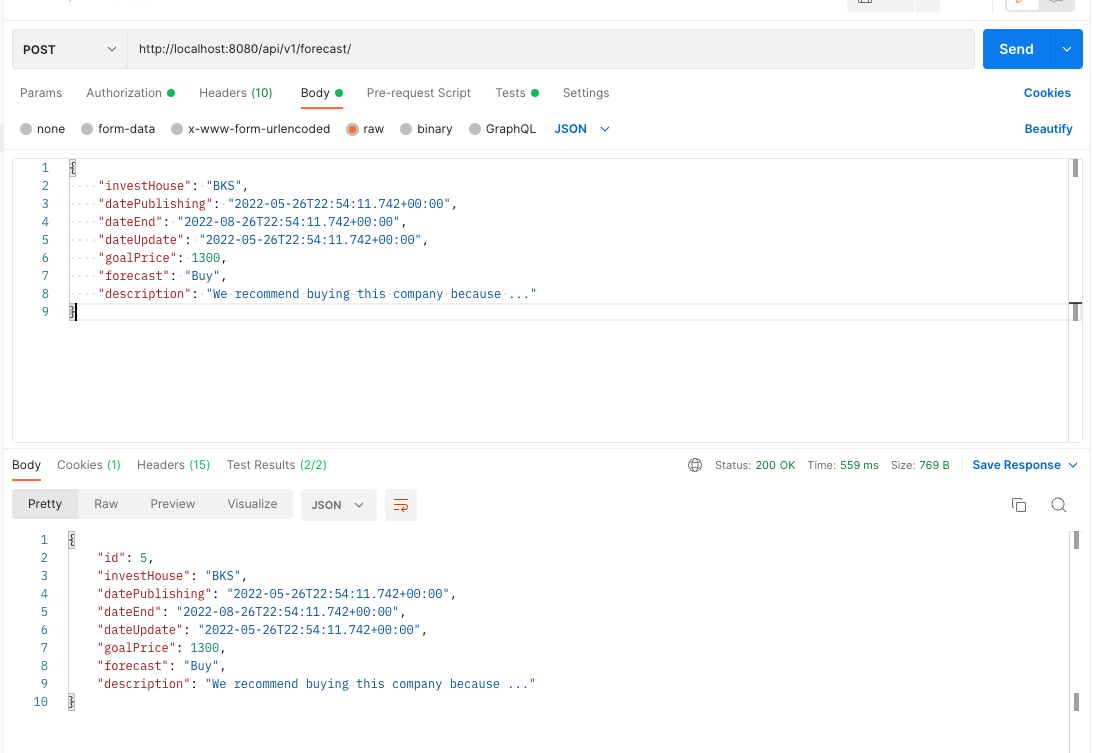
\includegraphics[scale=0.44]{inc/img/post.png}
	\end{center}
	\captionsetup{justification=centering}
	\caption{Пример добавления прогноза с помощью POST запроса.}
	\label{img:save-example}
\end{figure}
\newpage

\begin{figure}[h!]
	\begin{center}
		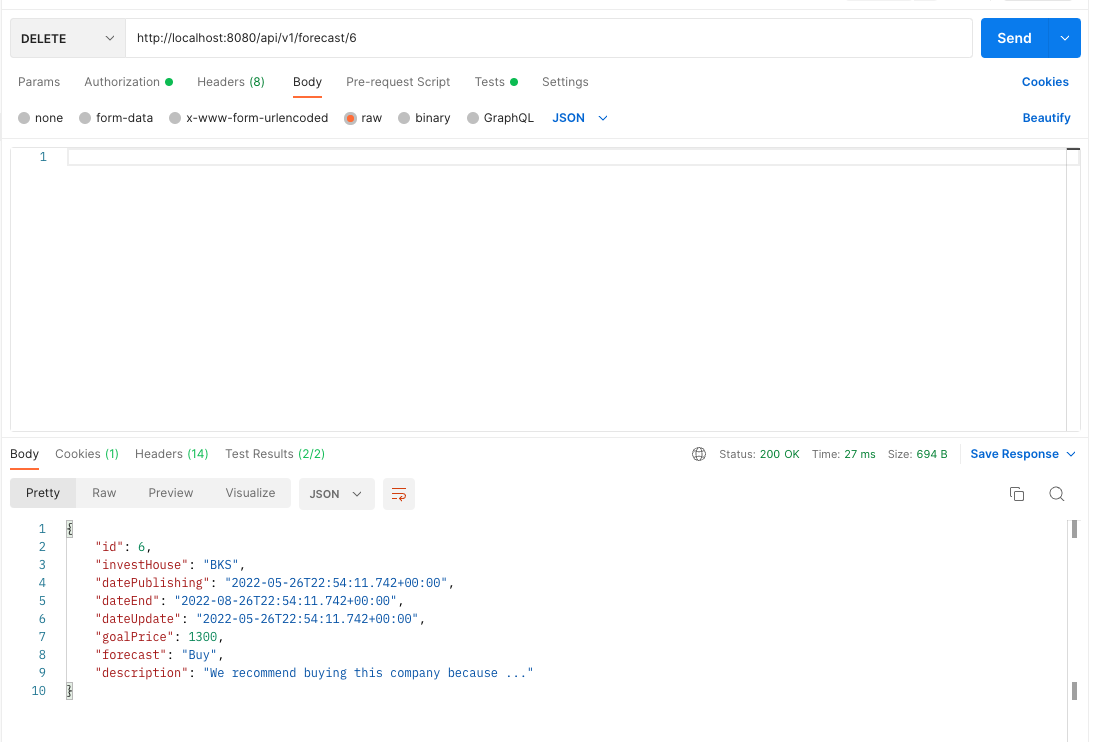
\includegraphics[scale=0.44]{inc/img/delete.png}
	\end{center}
	\captionsetup{justification=centering}
	\caption{Пример удаления прогноза с помощью DELETE запроса.}
	\label{img:delete-example}
\end{figure}

\newpage

\begin{figure}[h!]
	\begin{center}
		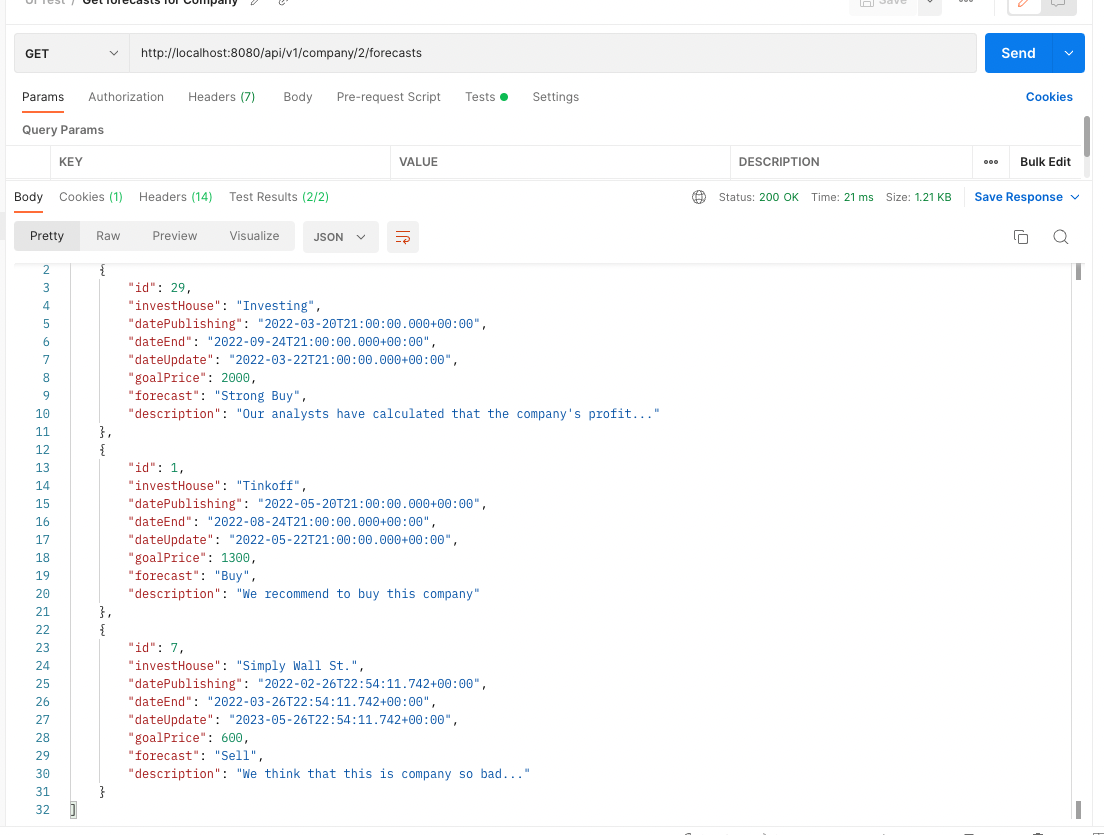
\includegraphics[scale=0.44]{inc/img/get.png}
	\end{center}
	\captionsetup{justification=centering}
	\caption{Получение всех прогнозов на компанию с \texttt{id = 2}}
	\label{img:get-example}
\end{figure}

\section*{Вывод}

В данном разделе были представлены средства реализации программного обеспечения, листинги ключевых компонентов системы, а также была продемонстрирована работоспособность программного обеспечения.